\section{Konzept}

\begin{frame}
	\frametitle{Konzeptauswahl}
	\frametitle{Finden geeigneter Algorithmen f�r das Gesamtsytem}
	\begin{beamerboxesrounded}[shadow=true]{Gesamtsystem bestehend aus:}
		\begin{itemize}[<+->]
			\item Sender bestehend aus:
				\begin{itemize}
					\item (Pseudo-)Zufallszahlengenerator (PRN-Schieberegister)
					\item Signalgenerator (DDS, CORDIC)
					\item Modulator (FSK)
				\end{itemize}
			\item Empf�nger bestehend aus:
				\begin{itemize}
					\item Bandpassfilter (1 je Tr�gerfrequenz)
					\item H�llkurvendemodulator (1 je Tr�gerfrequenz)
					\item Tiefpassfilter (1 je Tr�gerfrequenz)
					\item Vergleicher (mit Hysterese)
				\end{itemize}
			\item Weitere Schnittstellenmodule
			\item Fehlerkorrekturhilfen
		\end{itemize}
	\end{beamerboxesrounded}
\end{frame}

\begin{frame}
	\frametitle{Konzeptdiagramme}
		\begin{center}\footnotesize
			\begin{figure}
				  \centering
						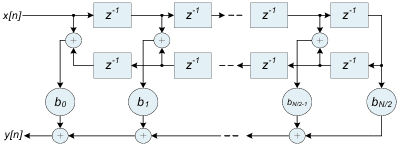
\includegraphics[width=0.8\linewidth]{bilder/FIRLinearphasenstruktur}
					\caption{FIR in Linearphasenstruktur}
			\end{figure}
		\end{center}
		\begin{center}
			\begin{figure}
				\begin{minipage}[b]{.45\linewidth}
					\centering
					  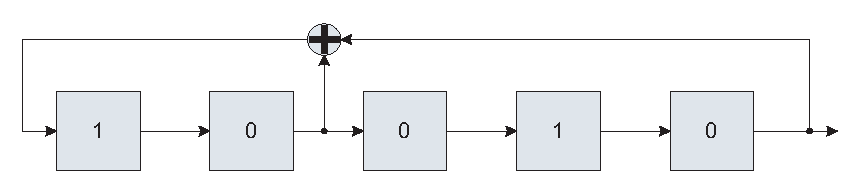
\includegraphics[width=0.9\linewidth]{bilder/prn_register}
					\caption{PRN-Register}
				\end{minipage}
				\begin{minipage}[b]{.45\linewidth}
				  \centering
						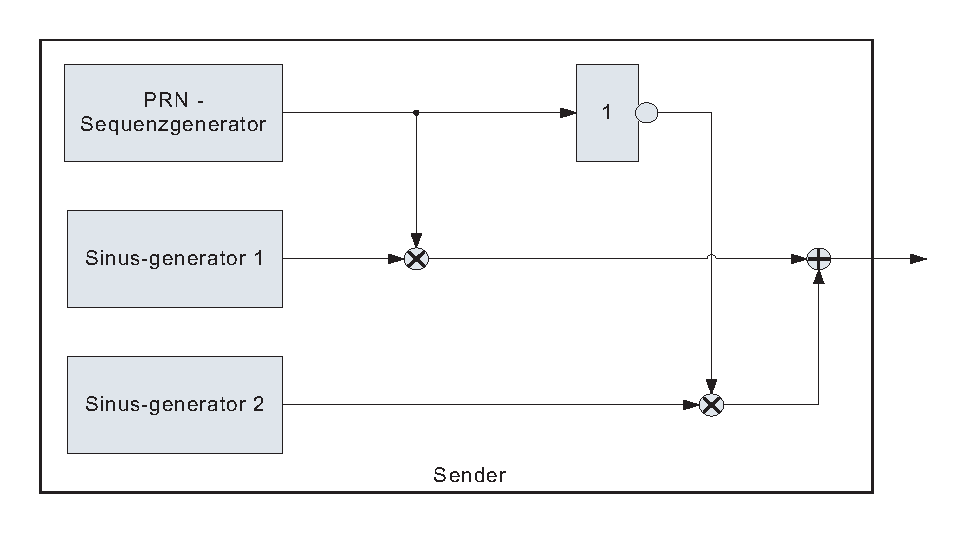
\includegraphics[width=0.7\linewidth]{bilder/sender_blockschaltbild}
					\caption{Sender Blockschaltbild}
				\end{minipage}
			\end{figure}
		\end{center}\normalsize
\end{frame}

\section{Entwickungsplattform}

\begin{frame}
	\frametitle{Entwicklungsplattform}
		\begin{beamerboxesrounded}[shadow=true]{M�glichkeiten:}
			\begin{itemize}[<+->]
				\item Rahmenbedingungen (aus Konzept)
				\item Kernkomponente FPGA
				\item Entwicklungssystem
				\begin{itemize}
					\item Verf�gbare Evaluierungsboards
					\item Design eines eigenen Systems
				\end{itemize}
			\end{itemize}
		\end{beamerboxesrounded}
		
		\only<6->{$\Rightarrow$ Eigendesign}
\end{frame}

\begin{frame}
	\frametitle{Entwicklungsplattform}
		\begin{beamerboxesrounded}[shadow=true]{Eigenes System:}
			\begin{itemize}[<+->]
				\item Rahmenbedingungen ($2 \cdot \approx 300$ \euro{}, $15 \cdot \approx 200$ \euro{})
				\item Auswahl geeigneter Bauteile
				\item Schaltplanerstellung
				\item Layout (Platzierung und Entflechtung)
				\item Aufbau
				\item Fehleranalyse
			\end{itemize}
		\end{beamerboxesrounded}
		
		\pause
		
		\begin{beamerboxesrounded}{3D-Modell des SPATES}
			\begin{center}
				\begin{figure}
					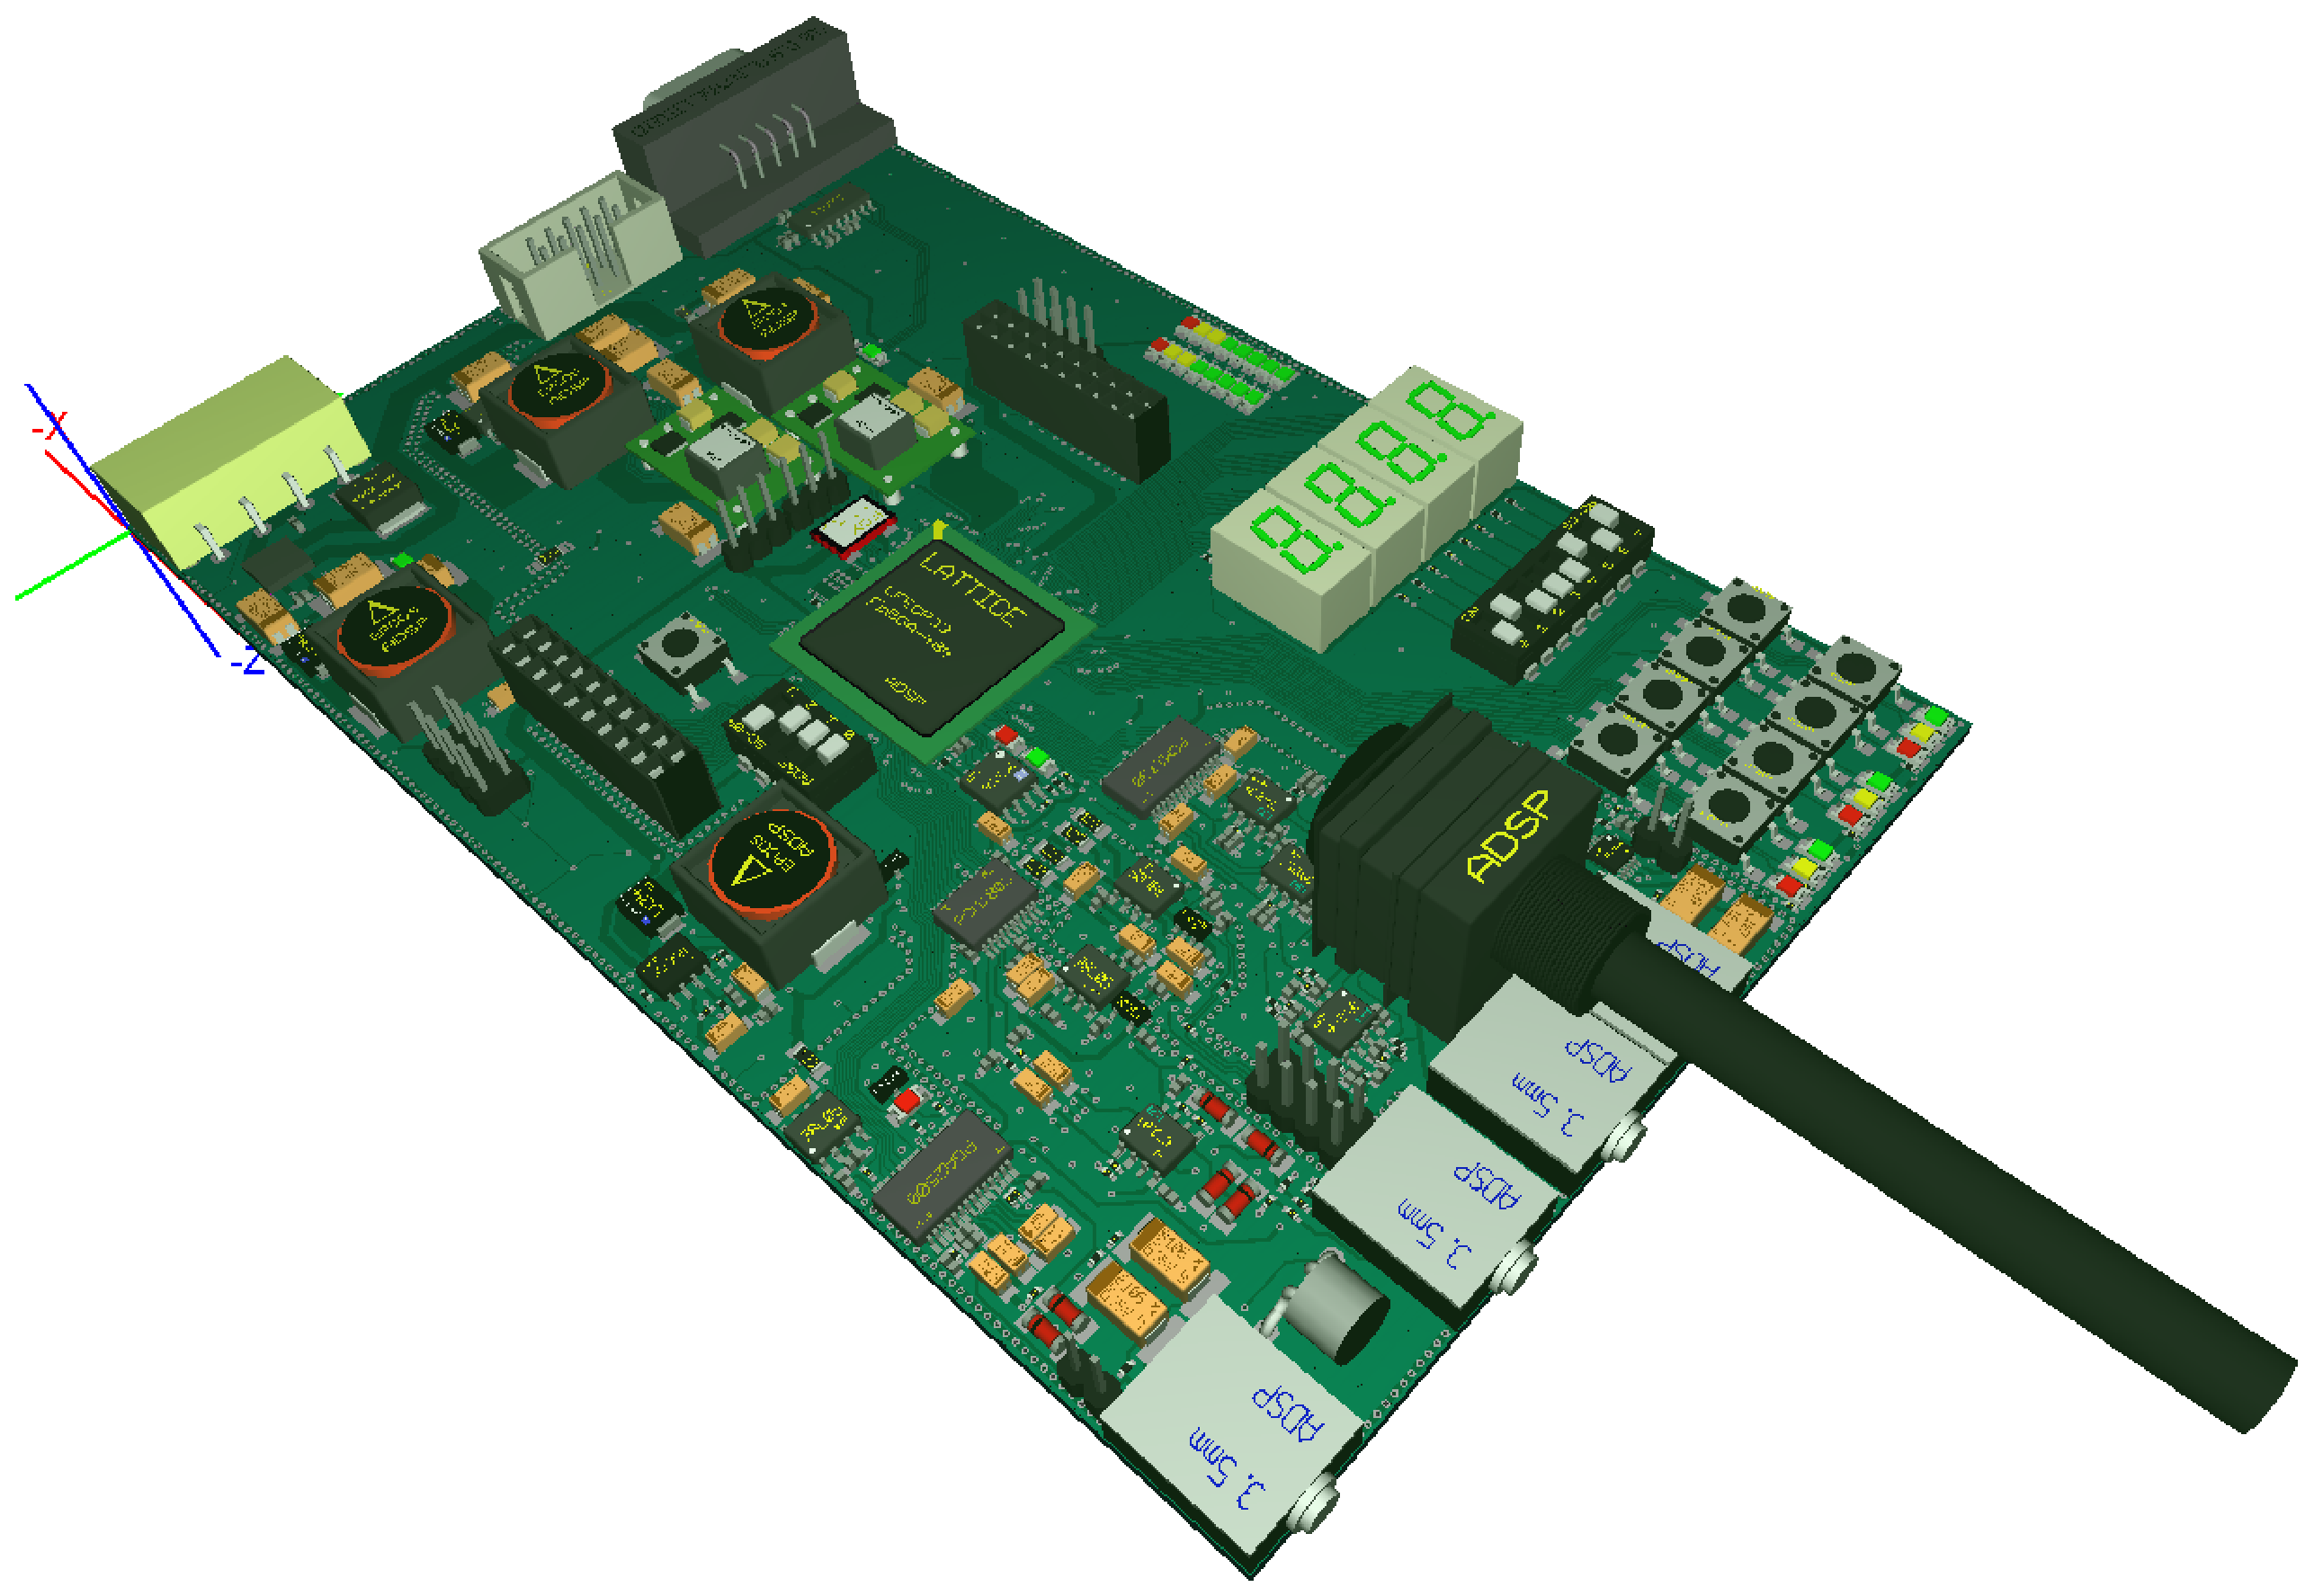
\includegraphics[width=0.6\linewidth]{bilder/ADSP-SPATES_schraeg_links_vorne}
				\end{figure}
			\end{center}
		\end{beamerboxesrounded}	

\end{frame}

\subsection{Praktikumskonzept}

\begin{frame}
	\frametitle{Praktikumskonzept}
	\framesubtitle{Abstraktion der Hardware}
	
	\begin{itemize}
		\item \alert{Grundlegend:} Starke Abstraktion der Hardware
		\item Aufbau des Wissens in kleinen Teilen
			\begin{itemize}[<+->]
				\item Vorgefertigtes Modul mit kleiner "`Leerstelle"'
				\item Grobe Vorgabe des inneren Toplevels
				\item Vorgabe der Ports
				\item V�llig selbst�ndige Programmierung der Aufgabe
			\end{itemize}
		\item Auf h�ufige Anf�nger-Fehler direkt hinweisen
	\end{itemize}
\end{frame}

\begin{frame}
	\frametitle{Abstraktionsmodell}
	\framesubtitle{Der Toplevel im Toplevel}
	\begin{beamerboxesrounded}{Hardwareabstraktion}
		\begin{center}
			\begin{figure}
				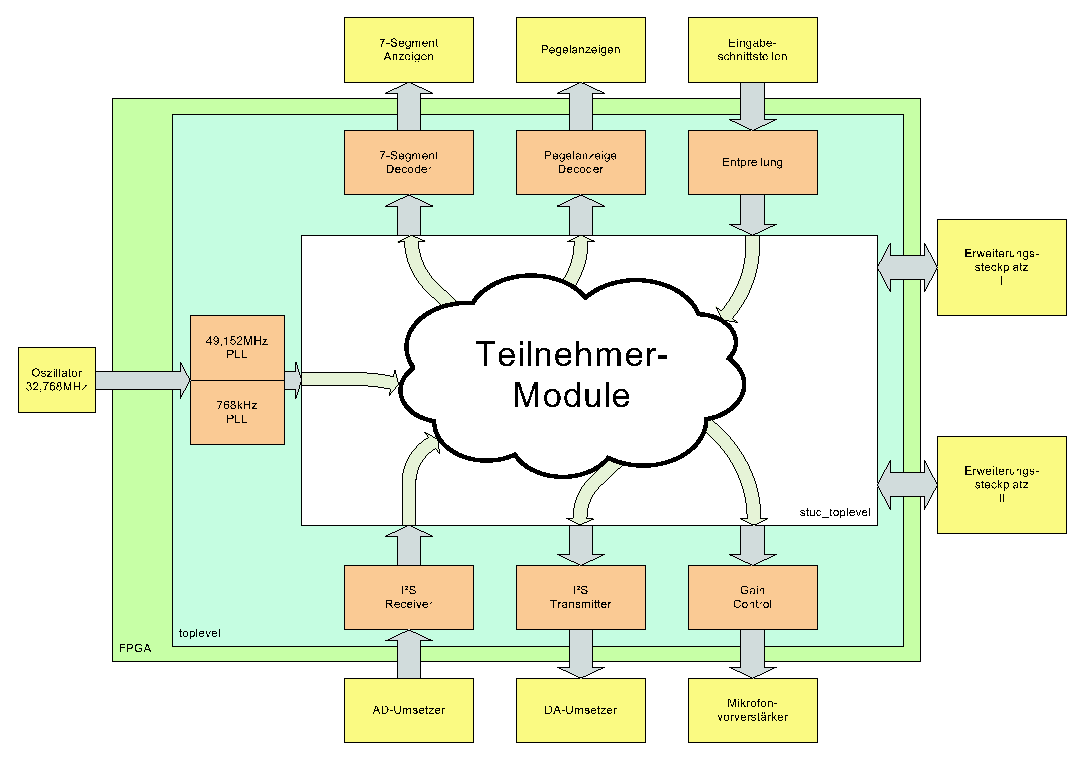
\includegraphics[width=0.8\linewidth]{bilder/hardwareabstraktion}
			\end{figure}
		\end{center}
	\end{beamerboxesrounded}	
\end{frame}